% !TeX root = ../libro.tex
% !TeX encoding = utf8

\chapter{Modules for Experiments in Stellar Astrophysics - MESA}\label{ch:cuarto-capitulo}
\section{Introducción}
Como hemos anticipado, la herramienta de evolución estelar MESA ha sido utilizada extensivamente en nuestra línea de investigación. Este simulador incorpora módulos que se actualizan de manera periódica en base a los avances derivados de los trabajos más novedosos sobre ecuaciones de estado, opacidad, velocidades de reacción nuclear, datos de difusión de elementos y condiciones de límite atmosférico. Es una herramienta muy versátil a la hora de poder contrastar las valores obtenidos con los resultados esperados por un determinado modelo, o para realizar predicciones a partir de nuevos modelos y contrastar sus pronósticos con los datos disponibles de otros trabajos de investigación.\par

En el caso particular de nuestra línea de investigación estamos interesados en estudiar los mecanismos que intervienen en la destrucción del litio en estrellas similares a nuestro Sol, y particularmente en ella. Resaltar nuevamente el hecho de que a día de hoy no existe una opinión unánime en la comunidad científica, más allá de que los modelos de evolución estelar no producen resultados coherentes con las observaciones, sobre cuáles son los mecanismos que gobiernan el proceso de agotamiento del litio estelar, y de cuándo se ponen en marcha o se detienen. Existen diversos planteamientos de procesos que intentan dar una respuesta a este enigma.\par 

En nuestra investigación nos centramos en cómo influyen en modelos de estrellas de tipo solar, aquéllos con 1.0 $\msun$ y con una metalicidad (Z) similar al Sol, los efectos de la rotación y de la pérdida de momento angular causada por la presencia de campos magnéticos que inducen un efecto de frenado magnético. Estos campos magnéticos tendrán, en una primera aproximación, una intensidad fija a lo largo de toda la evolución temporal del modelo. Posteriormente se extenderá el modelo para simular campos magnéticos de intensidad variable.\par

Adicionalmente, los modelos simulados se basan en la teoría de la longitud de mezcla (Mixing Length Theory, MLT) para modelar la convección estelar. Este formalismo depende del parámetro libre longitud de mezcla ($\amlt$), parámetro que mayoritariamente tiene un valor preestablecido y fijo durante toda la simulación. En nuestro trabajo, realizaremos simulaciones manteniendo estable el valor de $\amlt$ pero también introduciremos la posibilidad de hacerlo evolucionar temporalmente en base a otros parámetros estelares.\par

Una vez hemos definido el los objetivos principales a alcanzar, el siguiente paso lógico es definir una estrategia para poder alcanzarlos, y esta pasa por hacer uso de MESA. Al estudiar en detalle la funcionalidad que MESA\footnote{\url{http://mesa.sourceforge.net/release/2018/03/21/r10398.html}} oferta por defecto, se constata que el simulador no ofrece capacidades ni para la incorporación de campos magnéticos, ni para la variabilidad temporal del valor $\amlt$. Esto implica que, como parte de nuestra línea de investigación, debemos añadir como un nuevo objetivo la ampliación de las capacidades técnicas del simulador MESA. Adicionalmente, éste debe ser el primero a alcanzar antes de poder realizar las simulaciones adecuadas para nuestra línea de investigación.\par

El primer desafío a solventar es el de entender cómo incorporar las extensiones necesarias al simulador MESA. Al mismo tiempo, hay que respetar su estructura modular de manera que no provoquemos efectos colaterales indeseables en otros módulos y/o el resto de parámetros utilizados por el simulador. Para dar solución a este punto tenemos que basarnos en los planteamientos teóricos documentados en el Capítulo \ref{ch:tercer-capitulo} e implementarlos, en forma de rutinas en código Fortran, para que puedan ser utilizadas en conjunto con el resto de módulos de MESA. Por otra parte, se hace también necesario el comprender los diferentes parámetros y procesos que MESA utiliza a la hora de calcular las abundancias de los diferentes elementos que podemos encontrar en una estrella a lo largo de su evolución, tanto en su interior como en su atmósfera. Por tanto, aquí tenemos otra área de estudio que pasa por conocer las diferentes capacidades ya disponibles en el simulador que tengan impacto sobre el agotamiento del litio, entender cuándo pasan a ser relevantes en el proceso evolutivo de la estrella, cuáles son los parámetros que gobiernan su funcionamiento, las relaciones que guardan entre ellos y, por último, qué valores son los más recomendables para dar soporte al escenario de simulación que acabamos de plantear.\par

Una vez tengamos la parametrización adecuada para nuestro planteamiento teórico, pasaremos a simular de manera sistemática, haciendo uso de nuestras nuevas rutinas y de un conjunto de modelos con diferentes valores para sus parámetros relevantes: velocidad angular, intensidad del campo magnético y valor de $\amlt$. Los resultados de abundancia de litio que obtengamos en cada uno de los escenarios planteados los enfrentaremos con los que arroja MESA sin hacer uso de nuestra rutina. Esta comparación de resultados nos deberá de dar un primer indicio de si nuestro planteamiento realmente tiene algún efecto notable sobre la abundancia litio calculada por el simulador con y sin nuestras rutinas. Finalmente, en base a los valores obtenidos, analizaremos las consecuencias que nuestras rutinas han tenido sobre ellos y presentaremos una serie de conclusiones de por qué obtenemos estos datos y cómo se interpretan los mismos en base a los estudios teóricos y observaciones obtenidas por otras líneas de investigación.\par

\subsection{El proyecto MESA}
Como indica su contribuidor y desarrollador principal Bill Paxton \citep{Paxton2011, Paxton2013, Paxton2015, Paxton2018} MESA es un conjunto de librerías de código abierto, robustas y eficientes escritas en el lenguaje de programación Fortran 95 que es susceptible de ser utilizado en una amplia gama de aplicaciones en astrofísica estelar computacional. Está categorizado dentro de los denominados códigos de evolución estelar unidimensional (1-D) y combina un gran número de módulos numéricos y físicos que le permiten simular una amplia variedad de escenarios de evolución estelar, que van desde los que incluyen estrellas de muy baja masa hasta los que caracterizan estrellas masivas, además de tener en cuenta fases avanzadas de evolución, como el flash del helio, pulsos térmicos o la rama asintótica gigante (Asymptotic Giant Branch, AGB). Utiliza un modelo de malla o zonas adaptables, que representa las diferentes capas y celdas en las que se estructura el modelo estelar, y emplea sofisticados controles de evolución temporal.\par

MESA se caracteriza por resolver las ecuaciones de estructura y composición de forma simultánea. Incluye módulos con el último “estado del arte” capaces de resolver las ecuaciones de estado, opacidad, velocidades de reacción nuclear, difusión de elementos y condiciones de límite atmosférico necesarias para realizar la evolución estelar. Cada módulo está construido a partir de una biblioteca desarrollada en Fortran 95 y diseñada de forma modular, diferenciando entre una interfaz pública destinada a ser utilizada por otros módulos y una parte privada donde se implementa la lógica necesaria que permanece inaccesible al resto de módulos. Esta buena práctica permite desarrollar nuevos módulos o revisar los existentes de manera independiente.\par

MESA se basa en el principio de código abierto: cualquiera puede descargar el código fuente en el que se basa, compilarlo y ejecutarlo para sus propias necesidades de investigación, además de poder ampliar su funcionalidad, como se mostrará a lo largo del presente documento. El propósito de ser distribuido como código abierto es el de involucrar y llegar al mayor número de miembros de la comunidad astrofísica para que hagan uso de la herramienta, y al mismo tiempo alentarla para que hagan contribuciones al proyecto, ya sea en forma de pruebas, detección y corrección de errores o añadiendo nuevas capacidades al simulador.\par

\section{¿Cómo trabajar con MESA?}
Cuando se descarga e instala MESA (en el presente documento no entramos al detalle de cómo hacer esto) veremos que bajo el directorio de instalación existe una serie amplia de subdirectorios adicionales. La mayoría de ellos contienen el código para los diferentes módulos que componen MESA y que proporciona alguna funcionalidad específica. De todos ellos, el módulo más importante es \textit{star}, ya que es éste el módulo que interacciona y controla la ejecución de los demás. Adicionalmente, es también el módulo encargado de gestionar el estado interno de la estrella y de calcular el paso temporal a utilizar en cada iteración durante el proceso de simulación.\par

Por otra parte, MESA se apoya en ficheros de proyecto en los que se fijan los diferentes parámetros iniciales, bajo qué condiciones tiene que evolucionar la estrella, opciones de paradas y representación gráfica que deben utilizarse durante la simulación. MESA ofrece en su distribución un buen número de proyectos pre configurados para diferentes escenarios de evolución estelar.\par

\subsection{Fichero de configuración}
MESA utiliza el fichero \textit{inlist} como el punto de configuración y entrada para las simulaciones. Este fichero está compuesto de tres secciones principales. Cada una de ellas contiene un conjunto de opciones que controlan diferentes aspectos de MESA:
\begin{itemize}
    \item \textit{star\_job} - Sección con opciones que controlan cómo evoluciona la estrella
    \item \textit{controls} - Sección con opciones para el módulo \textit{star} de MESA
    \item \textit{pgstar} - Sección con opciones para la salida gráfica por pantalla
\end{itemize}

Las diferencias entre las secciones \textit{star\_job} y \textit{controls} pueden llegar a ser muy sutiles. Aun así, intentaremos dar unas reglas generales para tratar de averiguar en qué sección esperaríamos encontrar determinadas opciones de configuración.\par

La sección \textit{star\_job} contiene opciones relacionadas con la respuesta a preguntas como las siguientes:
\begin{itemize}
    \item ¿Cómo debería MESA obtener un modelo inicial a partir del que realizar la simulación?
    \item ¿Existe algún tipo de ajuste que MESA debería realizar sobre el modelo inicial?
    \item ¿Qué datos aplicables a la microfísica del simulador debe leer MESA?
    \item ¿Dónde debe almacenarse la salida de MESA?
\end{itemize}

Por otra parte, la sección \textit{controls} es la adecuada para opciones de configuración encaminadas a responder a las siguientes cuestiones:
\begin{itemize}
    \item ¿Cuándo se da por finalizada la simulación?
    \item ¿Qué procesos de transporte debe tener en cuenta MESA?
    \item ¿Qué tolerancias numéricas debe aplicar los métodos de resolución numérica que incorpora MESA?
\end{itemize}

Para conocer en más detalle las opciones, lo mejor es remitirse a la documentación estándar de MESA disponible en su sitio oficial\footnote{http://mesa.sourceforge.net}. Otra opción a nuestro alcance es la de consultar los ficheros de código donde se encuentran los valores por defecto asignados a cada una de las opciones del simulador, aunque para esto es recomendable poseer conocimientos en lenguajes de programación. Para cada una de las secciones comentadas anteriormente, MESA dispone de un fichero específico (\$MESA\_DIR hace referencia al directorio donde se encuentra instalado el software):

\begin{itemize}
    \item \$MESA\_DIR/star/defaults/star\_job.defaults
    \item \$MESA\_DIR/star/defaults/controls.defaults
    \item \$MESA\_DIR/star/defaults/pgstar.defaults
\end{itemize}

Las opciones tienden a estar agrupadas según la funcionalidad del módulo que regulan. Es recomendable que cuando se esté buscando una determinada opción, antes de entrar al detalle de cada una de las entradas en los ficheros, se intente identificar mediante las preguntas listadas anteriormente en qué fichero podríamos encontrarla y, una vez accedamos al contenido del mismo, revisemos las diferentes cabeceras disponibles a modo de comentarios que en ellos se encuentran.\par

\subsection{Controlando la salida} \label{sec:ctrl_salida}
MESA genera por defecto una cantidad ingente de información. Existen dos tipos de ficheros de salida con información de la simulación: uno con información histórica sobre cantidades globales (masa, luminosidad) almacenadas a diferentes intervalos de tiempo y otro tipo con perfiles del interior estelar que almacena información con cantidades que varían de forma espacial (densidad, presión) en un determinado instante de tiempo. El contenido de estos ficheros no se encuentra directamente accesible en el fichero \textit{inlist}, sino en los siguientes ficheros específicos para cada uno de ellos:

\begin{itemize}
    \item \$MESA\_DIR/star/defaults/history\_columns.list
    \item \$MESA\_DIR/star/defaults/profile\_columns.list
\end{itemize}

Los ficheros anteriores contienen las configuraciones por defecto que ofrece MESA. Si necesitamos modificar alguna de las opciones que aparece en ellos, lo recomendable es no hacerlo directamente sobre estos ficheros, sino hacer una copia de los mismos en nuestro directorio de trabajo y realizar las modificaciones oportunas en ellos.\par

Adicionalmente, si se diese la situación (como ha sido en nuestro caso) de que se quieran mostrar valores de propiedades diferentes a los que aparecen por defecto en alguno de estos dos ficheros, cabe la posibilidad de añadirlos haciendo uso, como veremos más adelante, del fichero \textit{run\_star\_extras.f}.\par

\section{¿Cómo extender MESA?}
A veces se hace necesario extender la funcionalidad de MESA porque la que viene por defecto en el simulador no cumple con las necesidades del problema que queremos abordar. Para estas situaciones, MESA ofrece la opción de ampliar su funcionalidad de un modo relativamente sencillo y elegante, y sin necesidad de tener que modificar el código fuente del simulador en sí. Con esto se garantiza que el mismo no queda alterado en su funcionamiento estándar a raíz de una alteración del código base, a la vez que permite que otros usuarios de MESA no tengan que alterar sus instalaciones para poder ejecutar simulaciones que hacen uso de funcionalidades no estándar. \par

MESA proporciona el archivo \textit{run\_star\_extras.f} que ofrece una variedad de puntos de extensión (\textit{hooks}) destinados a implementar acciones que no pueden hacerse únicamente mediante el uso del fichero de proyecto \textit{inlists}. Entre estas acciones adicionales tenemos la posibilidad de cambiar parámetros en cada paso de la simulación, o la de reemplazar muchas de las rutinas de física predeterminadas que trae el simulador.\par

\subsection{Activación de capacidades extras}
El primer paso para hacer uso de las capacidades extendidas de MESA es el de proceder a activarlas. Para ello debemos editar el fichero \textit{run\_star\_extras.f}. Veremos que el contenido del mismo es bastante simple, se limita a incluir otro fichero que es el que contiene el conjunto de rutinas predeterminadas que se entrega con MESA. Las rutinas definidas en ese fichero son las candidatas a ser personalizadas, pero lo haremos sin afectar a las versiones originales. Para ello, procederemos a reemplazar esta declaración de inclusión por el contenido del archivo referenciado, consiguiendo de este modo tener nuestra propia copia local y personal.\par

\subsection{Extensión mediante hooks}
MESA proporciona una forma de sustituir la mayoría de las rutinas físicas que ofrece por defecto sin la necesidad de, como apuntábamos anteriormente, tener que modificar el código original del programa mediante el uso de los denominados \textit{hooks} o puntos de extensión. Para ello se necesitan seguir los siguientes pasos:

\begin{enumerate}
    \item Activar el \textit{hook} deseado en el fichero \textit{run\_star\_extra.f} situado en el directorio \textit{src} del proyecto en el que estamos trabajando
    \item Indicar nuestra versión del módulo de física a sustituir/ampliar
\end{enumerate}

Seguidamente debemos localizar qué \textit{hook} nos interesa modificar de entre todos los que ofrece MESA. Lo primero que debemos hacer es conocer los que MESA pone a nuestra disposición. Un \textit{hook} no deja de ser más que un fichero escrito en Fortran que implementa un conjunto de rutinas numéricas relacionadas con un determinado proceso físico que se ejecuta durante la evolución de una estrella. Cada una de estas rutinas es susceptible de ser sustituida por una versión propia con nuestro planteamiento físico.\par

Los dos conceptos más importantes que se necesita saber a la hora de poder usar \textit{run\_star\_extras.f} de una manera efectiva son:
\begin{itemize}
    \item El flujo de control de un paso de ejecución de MESA
    \item El contenido de la estructura \textit{star\_info}
\end{itemize}

Las diferentes rutinas presentes en \textit{run\_star\_extras.f} se invocan en diferentes puntos durante la ejecución de MESA. En el Listado \ref{lst:bucle_ctrl}, y a modo de pseudo\-código en Fortran, podemos encontrar el aspecto del bucle principal de control sobre el que itera MESA. El corazón del simulador MESA es la sección \textit{step\_loop}. Es en ella donde se sitúa toda la maquinaria mediante la que MESA evalúa y resuelve las ecuaciones de la estructura estelar.\par

\begin{lstlisting}[language=Fortran, float, caption={Bucle de control principal sobre el que itera MESA en cada paso temporal}, label={lst:bucle_ctrl}]
subroutine run1_star(...)
  ! star is initialized here

  ! before evolve loop calls:
  !   extras_controls
  !   extras_startup
  call before_evolve_loop(...)

  ! evolve one step per loop
  evolve_loop: do while(continue_evolve_loop)
    call before_step_loop(...)

    ! may need to repeat this loop
    step_loop: do 
      if (stop_is_requested(s)) then
        continue_evolve_loop = .false.
        result = terminate
        exit
      end if

      result = star_evolve_step(...)
      if (result == keep_going) 
        result = star_check_model(...)
      if (result == keep_going) 
        result = extras_check_model(...)
      if (result == keep_going)
        result = star_pick_next_timestep(...)
      if (result == keep_going) 
        exit step_loop

      if (result == terminate) then
        continue_evolve_loop = .false.
        exit step_loop
      end if
    end do step_loop

    ! after_step_loop calls:
    !   extras_finish_step
    call after_step_loop(...)

    if (result /= keep_going) then
       exit evolve_loop
    end if

    ! write out data
    !
    ! do_saves calls:
    !   how_many_extra_history_columns
    !   data_for_extra_history_columns
    !   how_many_extra_profile_columns
    !   data_for_extra_profile_columns
    call do_saves(...)

   end do evolve_loop

   ! after_evolve_loop calls:
   !   extras_after_evolve
   call after_evolve_loop(...)
end subroutine run1_star
\end{lstlisting}

Por otro lado, en la estructura de datos \textit{star\_info}, MESA almacena toda la información sobre la estrella que está evolucionando. Por convención en el código, el nombre de la variable se utiliza a lo largo del mismo, incluyendo también el que aparece en \textit{run\_star\_extras.f} para hacer referencia a esta estructura\footnote{En Fortran, el operador de porcentaje (\%) se utiliza para acceder a los componentes de la estructura, así que s\% x hace referencia al campo x contenido en la estructura s.}.\par

La estructura \textit{star\_info} contiene el modelo estelar propiamente dicho, es decir, información sobre las zonas o capas que componen la estrella que se está simulando, su perfil termodinámico, perfil de composición, etc. También contiene todos los valores que hemos asignado a los parámetros que aparecen en el fichero de proyecto \textit{inlist}, así como los valores por defecto para el resto de parámetros físicos que no hemos indicado de forma explícita.\par

Además de todo lo que hemos comentado hasta ahora, MESA también pone a nuestra disposición un conjunto de listas de valores que nos facilitará el poder pasar parámetros fijados en el fichero \textit{inlist} del proyecto a nuestras rutinas de código. Estos vectores de elementos, con un tamaño máximo de 100 valores y que no forman parte del conjunto estándar de parámetros, son: \textit{x\_ctrl}, \textit{x\_integer\_ctrl}, y \textit{x\_logical\_ctrl} y nos permiten almacenar valores de tipo real, entero y lógico respectivamente (ver Listado \ref{lst:paso_params}).\par

\begin{lstlisting}[language=Fortran, float, caption={Paso de parámetros no estándar a través del fichero de proyecto inlist}, label={lst:paso_params}]
&controls
  x_ctrl(1) = 3.14
  x_ctrl(2) = 2.78
  x_integer_ctrl(1) = 42
  x_logical_ctrl(1) = .true.
/ ! end of controls inlist
\end{lstlisting}

\subsection{Extensión ficheros de salida}
Anteriormente hacíamos referencia a cómo controlar la información estándar que MESA ofrece a través de los dos tipos de fichero de salida: \textit{history} y \textit{profile} (ver Sección \ref{sec:ctrl_salida}). Adicionalmente a esta opción, tenemos la posibilidad de enviar a alguno de estos dos ficheros información que, o bien la calcula ya de por sí MESA pero no está pensada para ser volcada en estos ficheros, o bien puede representar valores que vienen derivados de nuestras rutinas y que, por lo tanto, no forman parte de la parametrización estándar de MESA.\par

Para cualquiera de los dos casos comentados existen un par de rutinas dentro del fichero \textit{run\_star\_extras.f} que nos permiten, mediante sencillas modificaciones en los métodos \textit{how\_many\_extra\_history\_columns} y \textit{data\_for\_extra\_history\_columns}, añadir cuántos parámetros queramos\footnote{En realidad, existe un máximo de 100 parámetros adicionales.} (ver Listado \ref{lst:extra_columns}). Para ello, simplemente hay que indicar la cantidad de nuevos parámetros en los que estamos interesados, el nombre de los mismos (ver Listado \ref{lst:extra_name_columns}) y de dónde obtener sus valores.\par

\begin{lstlisting}[language=Fortran, float, caption={Configuración del número de parámetros adicionales a incluir en el fichero de salida.}, label={lst:extra_columns}]
  integer function how_many_extra_history_columns(id, id_extra)
    integer, intent(in) :: id, id_extra
    integer :: ierr
    type (star_info), pointer :: s
    ierr = 0
    call star_ptr(id, s, ierr)
    if (ierr /= 0) return

    how_many_extra_history_columns = 43
  end function how_many_extra_history_columns
\end{lstlisting}

\begin{lstlisting}[language=Fortran, float, caption={Definición de los nombres de los campos adicionales a aparecer en el fichero de salida.}, label={lst:extra_name_columns}]
  subroutine data_for_extra_history_columns(id, id_extra, n, names, vals, ierr)
    integer, intent(in) :: id, id_extra, n
    character (len=maxlen_history_column_name) :: names(n)
    real(dp) :: vals(n)
    integer, intent(out) :: ierr
    integer :: i
    type (star_info), pointer :: s

    ierr = 0
    i = 0
    call star_ptr(id, s, ierr)
    if (ierr /= 0) return
    !if (s% use_other_torque .eqv. .true.) then
      !routine activated
      names(1) = 'activated'
      vals(1) = s% x_ctrl(25) 

      !magnetic field torque
      names(2) = 'B'
      vals(2) = s% x_ctrl(61)
      ...

      !alfven_r
      names(43) = 'alfven_r'
      vals(43) = s% x_ctrl(62)
    !end if

  end subroutine data_for_extra_history_columns

\end{lstlisting}

\begin{lstlisting}[language=Fortran, float, caption={Ejemplo de asignación de valores calculados para la zona convectiva a los parámetros extras definidos.}, label={lst:extra_name_columns}]
  subroutine other_torque_mag_brk(id, ierr)	
    ...
  
    !Routine activated
    s% x_ctrl(25) = activated

    !Convective zone info
    s% x_ctrl(26) = sz_info_ptr% top_radius / s% r(1)
    s% x_ctrl(27) = sz_info_ptr% bot_radius / s% r(1)
    s% x_ctrl(28) = sz_info_ptr% top_mass / s% m(1)
    s% x_ctrl(29) = sz_info_ptr% bot_mass/ s% m(1)
    s% x_ctrl(30) = sz_info_ptr% top_zone
    s% x_ctrl(31) = sz_info_ptr% bot_zone
    s% x_ctrl(32) = sz_info_ptr% top_vrot
    s% x_ctrl(33) = sz_info_ptr% bot_vrot
    s% x_ctrl(34) = sz_info_ptr% top_omega
    s% x_ctrl(35) = sz_info_ptr% bot_omega
    ...
  
  end subroutine other_torque_mag_brk
\end{lstlisting}


\section{Módulos de interés de MESA}
Para empezar, vamos a enumerar los módulos de MESA que hemos encontrado de especial relevancia a estudiar para los objetivos de nuestra línea de investigación. Principalmente hemos basado nuestra búsqueda en localizar aquéllos que pueden tener relación directa con los procesos de destrucción del litio o con las reacciones nucleares que se producen en el interior estelar. Para cada uno de ellos ofrecemos un pequeño resumen.

\subsection{Módulo químico - chem}
El módulo \textit{chem} MESA está compuesto de una colección de datos, funciones y subrutinas encaminadas a la gestión de los elementos químicos y sus isótopos. Contiene información básica sobre cada uno ellos, desde el hidrógeno hasta el uranio. Adicionalmente incluye rutinas para realizar conversiones entre pesos, números atómicos y el nombre de los isótopos. Contiene listados completos sobre las abundancias solares de los diferentes elementos según diferentes estudios (para más información ver \cite{Paxton2011}).\par

\subsection{Reacciones termonucleares – rates}
El módulo \textit{rates} contiene los cocientes de reacciones termonucleares de \cite{Caughlan1988}, y \cite{Angulo1999}, siendo esta última opción la utilizada por defecto \citep{Paxton2011}. El conjunto de cocientes de reacciones incluido abarca más de 300 elementos e incluye las reacciones débiles necesarias para la quema de hidrógeno (emisión de positrones y captura de electrones), así como las reacciones de conversión neutrón-protón.

\subsection{Reacciones nucleares – net} \label{reac_nuc}
El módulo \textit{net} implementa redes de reacción nuclear. Por defecto, incluye una red básica de 8 isótopos: \isotope[1]{H}, \isotope[3]{He}, \isotope[4]{He}, \isotope[12]{C}, \isotope[14]{N}, \isotope[16]{O}, \isotope[20]{Ne}, \isotope[24]{Mg}, y otras extendidas para cálculos más detallados incluyendo el ciclo CNO, captura de partículas $\alpha$ y reacciones de captura protónica. Además de utilizar las redes existentes, MESA nos permite definir nuestras propias redes de reacción construidas a partir de las ya existentes (opción más sencilla) o completamente desde cero \citep{Paxton2011}.\par

Como indicaremos más detalladamente cuando analicemos la configuración final del fichero de proyecto \textit{inlist}, las reacciones que más nos interesan son las de las cadenas protón-protón en sus variantes I, II y III (ver Sección \ref{sec:li_reac_nuc} para más detalles).\par

\subsection{Teoría de longitud de mezcla – mlt}
El módulo \textit{mlt} implementa la teoría de longitud de mezcla estándar (MLT) \citep{Paxton2011}. En la dinámica de fluidos, MLT es una parametrización que intenta describir la transferencia de calor y material causado por una inestabilidad convectiva en el seno de un fluido. Este modelo ha sido utilizado en numerosos campos, incluyendo la ciencia atmosférica, oceanografía y estructura estelar, que es el caso que nos atañe. La longitud de mezcla se define como la distancia recorrida por una celda o burbuja de material sometida a una inestabilidad térmica convectiva.\par

\subsection{Módulo de difusión – diffusion} \label{subsec_diffusion}
El módulo \textit{diffusion} lo utiliza MESA para calcular la difusión de partículas y la sedimentación gravitacional resolviendo las ecuaciones de Burger \citep{Burgers1969} a través del método propuesto por \cite{Thoul1993}. El módulo de difusión trata los elementos presentes en el modelo estelar como pertenecientes a clases definidas por el usuario en términos de rangos de masas atómicas. Para cada clase, el usuario especifica un isótopo representativo y todos los miembros de esa clase son tratados idénticamente, con sus velocidades de difusión determinadas por el isótopo representativo. La rutina utiliza la fracción de masa de la clase correspondiente para obtener su coeficiente de difusión \citep{Paxton2015}. Como detallaremos más adelante, esta opción por defecto del módulo no es la más adecuada para obtener las abundancias de litio.\par

El cálculo de la difusión puede restringirse a zonas en las que la temperatura es superior a un valor mínimo o en las que la fracción de masa del elemento indicado es superior a cierto umbral.\par

\subsection{Otros parámetros de interés}
Además de los módulos listados anteriormente existen otra serie de parámetros que ofrece MESA que están relacionados también con el planteamiento teórico de nuestra investigación. En concreto nos estamos refiriendo a los parámetros de masa estelar, contenido de \isotope[1]{H}, \isotope[3]{He} y \isotope[4]{He} presente en la nube protoestelar, así como la metalicidad (Z) de la misma.\par
 
Finalmente, también tendremos en cuenta la rotación superficial de la estrella, ya que, como se ha venido comentando, este fenómeno físico es considerado un factor que influye en el agotamiento del litio, tanto potenciándolo, como llegando a inhibirlo.\par

\section{¿Cómo visualizar los resultados de MESA?}
\subsection{Visualización con pgstar}
Observar y analizar el resultado de las simulaciones atendiendo únicamente a los valores numéricos recogidos en los ficheros de salida no es la mejor opción a la hora de hacernos una idea de cómo están yendo nuestras simulaciones. Al menos, este es el caso en las etapas iniciales donde nuestra atención está más en saber si las simulaciones se están comportando de la manera esperada, o si por al contrario muestra una evolución no esperada. En este contexto, \textit{pgstar} es una herramienta extremadamente útil.

La herramienta \textit{pgstar} se encuentra integrada dentro de MESA y permite, a la vez que nuestra simulación se está ejecutando, la representación visual de un buen número de gráficas\footnote{Visitar https://docs.mesastar.org/en/latest/using\_mesa/using\_pgstar.html para obtener información complementaria.} generadas a partir de los datos de perfiles y valores temporales que se van produciendo. Entre éstas se encuentran diagramas HR, de abundacia de elementos químicos, de gravedad superficial vs. temperatura efectiva, por citar algunas de las posibilidades. La herramienta ofrece una gran flexibilidad a la hora de especificar tamaños de gráfica, número de ellas, fuentes, colores, leyendas y un sin fin de opciones adicionales. En el Listado \ref{lst:pg_star_config} se muestra un ejemplo de configuración de la herramienta para producir la gráfica de abundancia mostrada en la Figura \ref{fig:abundances}.


\begin{lstlisting}[language=Fortran, float, caption={Ejemplo de configuración de la herramienta pgstart para la generación de una gráfica de abundacias de elementos químicos.}, label={lst:pg_star_config}]
  ...	
  Abundance_win_flag = .true.
  Abundance_show_photosphere_location = .true.
  num_abundance_line_labels = 1

  Abundance_num_isos_to_show = 5
  Abundance_which_isos_to_show(1) = 'h1'
  Abundance_which_isos_to_show(2) = 'he4'
  Abundance_which_isos_to_show(3) = 'li7'
  Abundance_which_isos_to_show(4) = 'be7'
  Abundance_which_isos_to_show(5) = 'fe56'
  
  Abundance_log_mass_frac_min = -30
  Abundance_log_mass_frac_max = 10
  Abundance_file_interval = 1
  ...
  
\end{lstlisting}


\subsection{Visualización con terceras herramientas}
En determinadas ocasiones, las opciones de visualización ofrecidas por MESA no son las más adecuadas o convenientes para nuestros propósitos. Quizás porque no muestra el parámetro en el que estamos interesados, o si lo hace, deseamos otro tipo de formato de visualización. Aunque en la mayoría de los casos, la necesidad de recurrir a terceras herramientas para la visualización se debe a que necesitamos realizar algún tipo de preprocesamiento (ver Sección \ref{sec:gemelos_solares} para más detalles) sobre los mismos antes de proceder a su representación e interpretación final.\par

En nuestra investigación hemos recurrido a la herramientas Octave (ver Sección \ref{sec:tool_octave}) para la extracción, transformación, filtrado, enriquecimiento y visualización de los datos. En Octave establecemos un flujo de trabajo sobre los ficheros de salida de MESA, cuyas etapas más relevantes son:
\begin{enumerate}
	\item Extracción de datos - En esta fase, extraemos los datos de los ficheros de salida de MESA. El objetivo es obtener los datos brutos arrojados por el simulador para su posterior procesamiento.
	\item Transformación de datos - Los datos extraídos se someten a una serie de transformaciones para limpiarlos, enriquecerlos y estructurarlos de manera coherente. Las tareas comunes de transformación incluyen:
	\begin{enumerate}
		\item Limpieza de datos - Eliminación de valores nulos, corrección de errores y estandarización
		\item Conversión de formatos - Cambio de tipos de datos, ajuste de formatos de fecha, etc
		\item Agregación - Resumen de datos mediante cálculos (por ejemplo, sumas, promedios)
		\item Derivación - Creación de nuevas columnas a partir de las existentes (por ejemplo, calcular velocidades radiales a partir de las angulares)
	\end{enumerate}
	\item Carga -  En esta fase, los datos transformados pasan a ser visualizados en diferentes tipos de gráficas y quedan almacenados para su posterior interpretación. 
\end{enumerate}

\section{Extendiendo MESA - Parte I} \label{mesa_parte1}
Una vez obtenida una visión relativamente aceptable de las capacidades del simulador, la etapa a considerar es la de obtener un marco de referencia para nuestras simulaciones. Éste nos debe de asistir en la consecución de los siguientes objetivos:

\begin{itemize}
    \item Obtener la soltura suficiente con la herramienta, en lo que se refiere a su funcionamiento y parametrización, con el fin de obtener un punto de partida que nos sirva de referencia a la hora de comprobar los resultados obtenidos al incorporar nuestras rutinas
    \item Extender la funcionalidad del simulador MESA para que éste sea capaz de simular la presencia de campos magnéticos, tanto de intensidad fija como variable, el frenado magnético que estos producen, así como la evolución del parámetro $\amlt$ en la evolución de su estrella anfitriona
\end{itemize}

Con estos dos objetivos principales en mente, la concepción de los diferentes escenarios de simulación se realizó de forma condicionada al planteamiento teórico que introduciremos en el capítulo \ref{parte1}. En particular, estos escenarios soportan los siguientes procesos/características que intervienen, de alguna u otra forma, en la evolución de las abundancias de litio:

\begin{enumerate}
    \item Reacciones nucleares en las que interviene el litio
    \item Metalicidad y velocidad de rotación de la estrella
    \item Procesos de difusión
    \item Procesos de sedimentación
    \item Presencia de campo magnético de intensidad fija
\end{enumerate}

A la hora de extrapolar el subyacente teórico de nuestra línea de investigación a los escenarios de simulación, se opta por hacer una división en base al soporte que ofrece MESA de manera estándar para los conceptos teóricos que hemos acabado de enumerar y para aquéllos que no. De esta forma, nos encontramos que a excepción del punto 5, el resto se encuentran soportados por MESA. A partir de esta división se establecieron dos líneas de trabajo complementarias. La primera encaminada a simular los procesos teóricos 1-4 ya soportados por MESA, y una segunda, más avanzada, encaminada a extender el simulador con nuestra propia rutina de frenado magnético.\par

\subsection{Simulaciones acordes al marco teórico estándar de MESA}
En esta línea de trabajo nos centramos en hacer uso de las funciones y parametrizaciones estándar que ofrece MESA para dar soporte a los puntos teóricos 1-4 enumerados anteriormente y que recogemos de nuevo aquí:

\begin{enumerate}
    \item Reacciones nucleares en las que interviene el Li
    \item Metalicidad y velocidad de rotación de la estrella
    \item Procesos de difusión
    \item Procesos de sedimentación
\end{enumerate}

Como estamos interesados en observar cómo actúan esos procesos y parámetros físicos sobre la abundancia de litio en las fotosferas de estrellas de tipo solar (1.0 $\msun$) a lo largo de su evolución desde la PMS hasta la TAMS, nuestros modelos de simulación comienzan por fijar los siguientes parámetros:

\begin{enumerate}
    \item Establecer una metalicidad similar al Sol
    \item Detener la simulación al alcanzar la TAMS
    \item Obtener las abundancias para los elementos H, He, Li
\end{enumerate}

La composición química del Sol, incluyendo su metalicidad y masa inicial del modelo queda fijada por medio de los siguientes parámetros (ver Listado \ref{lst:ini_params}) de MESA:

\begin{lstlisting}[language=Fortran, float, caption={Parametrización de la metalicidad y masa inicial de la estrella}, label={lst:ini_params}]
  &star_job
    ! Solar composition, 
    set_uniform_initial_composition = .true.
    initial_h1 = 0.715399992
    initial_h2 = 1.430799984e-05
    initial_he3 = 4.48623528494e-05
    initial_he4 = 0.270255137647

    ! set metal fractions z fractions
    initial_zfracs = 6 ! AGSS09_zfracs

  &controls
    ! starting specifications
    ! or 1.0d0 in Msun units
    initial_mass = 1.0d0 
\end{lstlisting}

Posteriormente necesitamos indicar la condición de parada en la TAMS. Este momento en la evolución de una estrella queda asociado a la etapa en la que la estrella abandona la MS al haber agotado prácticamente todo el H que se encontraba en su núcleo. MESA nos ofrece la posibilidad establecer una condición de parada cuando las abundancias de ciertos elementos en el núcleo de la estrella alcanzan un cierto valor máximo o mínimo. En nuestro caso, utilizamos esta opción para indicar que cuando la abundancia del isótopo \isotope[1]{H} caiga por debajo de 0.000000001, la simulación se detenga (ver Listado \ref{lst:stop_params}).\par

Para poder obtener las abundancias de litio al final de la TAMS, primeramente necesitamos conocer qué reacciones nucleares son las responsables de su creación y si éstas están o no incluidas por defecto en la configuración de MESA. Como se adelantó en la sección \ref{sec:li_reac_nuc}, estas reacciones son las de cadena protón-protón en sus variantes I, II y III.\par

\begin{lstlisting}[language=Fortran, float, caption={Parametrización de la condición de parada de la simulación cuando se produce el agotamiento de H en el núcleo de la estrella}, label={lst:stop_params}]
&controls
  ! stop when the center mass fraction of 
  ! h1 drops below this limit
  xa_central_lower_limit_species(1) = 'h1'
  xa_central_lower_limit(1) = 1d-9
\end{lstlisting}


Por tanto, ya tenemos identificas la red de reacciones a activar en la configuración de MESA. Es en este punto donde volvemos a hacer referencia al módulo \textit{net} (ver Sección  \ref{reac_nuc}). Si recordamos, se indicaba que MESA viene pre configurado con una red de reacciones nucleares en las que sólo trata con 8 isótopos. Si queremos incluir más, debemos modificar la red inicial por otra que los incluya.\par

Con los parámetros anteriores incluidos en el proyecto, indicamos a MESA que sustituimos la red de reacciones nucleares por defecto por una nueva denominada \textit{mesa\_49.net} (ver Listado \ref{lst:mesa49}). Las redes son simples ficheros de texto en los que se indica al simulador las reacciones nucleares que debe tener en cuenta y cuál es el aspecto de éstas. En concreto, en la elegida se soportan, entre otras, las reacciones protón-protón en sus variantes I, II, III.\par

\begin{lstlisting}[language=Fortran, float, caption={Red de reacciones mesa\_49.net. Esta red incluye un tratamiento detallado de la para los elementos ligeros H, He, Li y Be}, label={lst:mesa49}]
  add_isos_and_reactions(
    neut
    h  1  2  ! hydrogen
    he 3  4  ! helium
    li7      ! lithium
    be7
    be 9 10  ! berylium
    b8       ! boron
    c 12 13  ! carbon
    n 13 15  ! nitrogen
    o 14 18  ! oxygen
    f 17 19  ! fluorine
    ne 18 22 ! neon
    na 21 24 ! sodium
    mg 23 26 ! magnesium
    al 25 27 ! aluminum
    si 27 30 ! silicon
    p 30 31  ! phosphorus
    s 31 34  ! sulfur
  )

  add_isos(
    ca40 ! calcium
    ti48 ! titanium
    fe56 ! iron
 )
\end{lstlisting}


Continuando con el marco físico a simular, pasamos a centrarnos en la activación de los mecanismos que, acorde a la teoría, tienen influencia en el agotamiento del litio:
\begin{itemize}
    \item Proceso de difusión
    \item Proceso de rotación
\end{itemize}

Como ya se indicaba en el apartado \ref{subsec_diffusion}:
\begin{center}
    \begin{minipage}{0.9\linewidth}
        \vspace{5pt}%margen superior de minipage
        {\small
        (MESA) calcula la difusión de partículas y la sedimentación gravitacional resolviendo las ecuaciones de Burger a través del método propuesto por Thoul \citep{Thoul1993}. El módulo de difusión trata los elementos presentes en el modelo estelar como pertenecientes a clases definidas por el usuario en términos de rangos de masas atómicas.
        }
        \vspace{5pt}%margen inferior de la minipage
    \end{minipage}
\end{center}

Activando la difusión en MESA también activamos la sedimentación gravitacional. De manera indirecta, queda también involucrado el módulo \textit{mlt}. Recordamos que este módulo es el encargado de calcular los coeficientes de difusión que entran en juego en el proceso de mezclado producido a consecuencia de los movimientos convectivos que se produce en el interior de la estrella.\par

Cabe también mencionar el tratamiento por clases que realiza MESA. Los isótopos presentes en nuestra red de reacciones nucleares que tienen un peso atómico similar son tratados de forma conjunta por la rutina de difusión en lo que se refiere a su velocidad de difusión. Ésta queda determinada por el isótopo representativo de la clase. La agrupación en clases tiene la ventaja de que las simulaciones se ejecutan de una manera más rápida ya que se ahorran cálculos. Por otra parte, tiene el inconveniente de que los resultados pueden llegar a ser menos exactos. En este trabajo hemos optado por desactivar la agrupación en clases a costa de aumentar los tiempos de simulación.\par

Una vez activada la nueva red de reacciones nucleares en nuestro fichero de proyecto MESA, conseguimos obtener las abundancias para el litio, las cuales son informadas en los ficheros de salida estándar que genera MESA. Adicionalmente estamos interesados en obtener el perfil de evolución de estos elementos a lo largo del tiempo de evolución de la estrella y en función del radio de la estrella (ver Figura \ref{fig:abundances}). Para ello recurrimos a utilizar las capacidades gráficas de MESA y mostramos la abundancia de estos elementos. Dado que sus concentraciones son muy pequeñas en comparación al H, debemos de proceder a ajustar el eje de abscisas del gráfico.\par

Adicionalmente, configuramos MESA para que, a cada paso en la simulación y para cada celda, tenga en cuenta si se producen o dejan de existir isótopos a consecuencia de las reacciones nucleares que están teniendo lugar. Dados los valores de abundancias tan pequeños que se obtienen para el litio, del orden de -20 respecto al logaritmo de la masa total de la estrella, optamos por activar el tratamiento de las reacciones nucleares sea lo más riguroso y exacto posible.\par

\begin{figure}
	\centering
	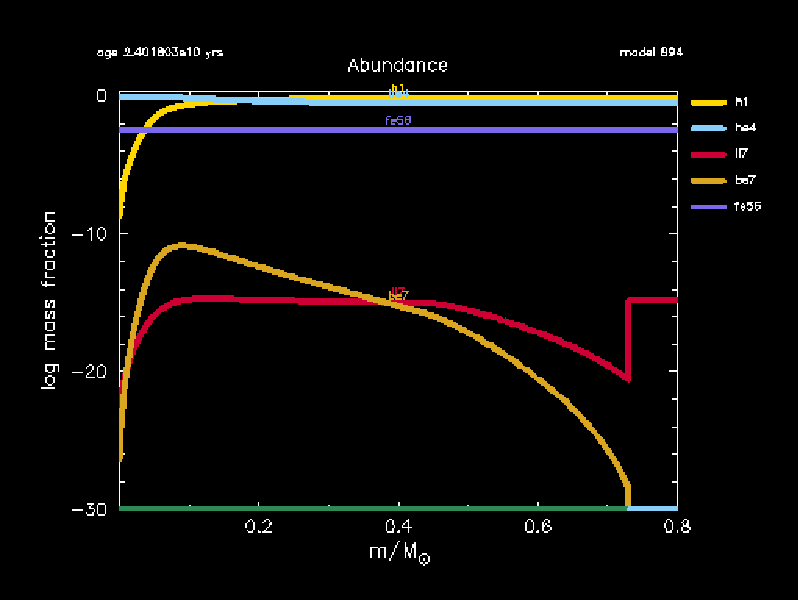
\includegraphics[width=0.5\textwidth]{img/tesis/abundances.pdf}
	\caption {Gráfica de abundancias en la que aparecen los elementos H, He, Fe, Li y Be. El eje de abscisas ha sido reescalado para posibilitar la representación de la abundancia de litio y berilio.}
	\label{fig:abundances}
\end{figure}


En lo que se refiere a la rotación de las capas superficiales de la estrella, MESA permite especificar una velocidad en km/s, que en nuestro caso ha quedado fijada en 20 km/s al ser un valor similar al que tenemos en el Sol. En el Listado \ref{lst:li_evol} mostramos la configuración adicional a añadir al proyecto de MESA para poder simular los conceptos teóricos discutidos hasta este momento.

\begin{lstlisting}[language=Fortran, float, caption={Parametrización de los procesos relacionados con el tratamiento del litio y su evolución temporal.}, label={lst:li_evol}]
&star_job
  ! Change default net in order to include 
  !reactions for Li
  change_initial_net = .true.
  new_net_name = 'mesa_49.net'
  ! If enable_adaptive_network is true, 
  ! then at each step, 
  ! the system calculates a new set of isos. 
  ! This can cause significant slowdowns
  enable_adaptive_network = .true.

  ! Activate surface rotation and set velocity
  change_v_flag = .true.
  new_v_flag = .true.
  set_initial_surface_rotation_v = .true.
  new_surface_rotation_v = 20 ! km/sec 

  ! Rotation off until near ZAMS
  change_rotation_flag = .false.
  new_rotation_flag = .true.

&controls
  ! toggle element diffusion
  do_element_diffusion = .true.
  ! If true, don't lump elements into 
  ! classes for diffusion. 
  ! Instead, each isotope in the network 
  ! is treated as its 
  ! own separate class. This can cause 
  ! significant slowdowns 
  ! for large nets, so it is off by default.
  diffusion_use_full_net = .true.
  diffusion_use_cgs_solver = .false.

&pgstar
  ! show HR diagram
  ! this plots the history of L,Teff 
  ! over many timesteps
  HR_win_flag = .true.

  ! configure file output 
  HR_file_flag = .true.
  HR_file_interval = 1


  ! show the abundance profile
  Abundance_win_flag = .true.
  num_abundance_line_labels = 1

  ! set how many elements must be shown
  Abundance_num_isos_to_show = 5
  Abundance_which_isos_to_show(1) = 'li7'
  Abundance_which_isos_to_show(2) = 'be7'
  Abundance_which_isos_to_show(3) = 'h1'
  Abundance_which_isos_to_show(4) = 'he4'
  Abundance_which_isos_to_show(5) = 'fe56'

  ! set the max and min value for the y-axis
  Abundance_log_mass_frac_min = -30
\end{lstlisting}

Hasta aquí, hemos conseguido obtener una configuración de proyecto base que recoge las características esenciales de la estrella a simular en MESA: pone en marcha los procesos físicos relacionados con la evolución del litio y es capaz de informar, tanto a través de los ficheros de salida estándar como de las representaciones gráficas, sobre las abundancias de este elemento a lo largo de la evolución de la estrella en sus etapas de PMS y MS. Esta configuración de proyecto y los valores arrojados por la simulación que lo utiliza, nos servirán para establecer el marco de referencia contra el que comparar los valores obtenidos en las nuevas simulaciones que extienden la funcionalidad de MESA.\par


\subsection{Simulaciones extendiendo el marco teórico estándar de MESA}
Una vez que hemos llegado a un punto en el que tenemos una configuración de proyecto que nos permite obtener las abundancias de litio de forma detallada, y además hemos conseguido activar los procesos de difusión y rotación superficial en nuestro modelo, damos paso a una segunda línea de trabajo consistente en extender el funcionamiento de MESA para incorporar nuestras propias rutinas de al simulador. Las consideraciones previas a tener en cuenta son las siguientes:

\begin{enumerate}
	\item Definir el formalismo matemático que soporta el proceso a incorporar a MESA
	\item Identificar los parámetros fijos y variables del formalismo
	\item Mapear los parámetros variables a sus equivalentes en MESA
	\item Identificar el \textit{hook} de MESA adecuado para incluir la rutina
	\item Implementar la rutina y asegurar su compatibilidad con MESA
	\item Identificar los parámetros de configuración
	\item Mapear los parámetros de configuración en el fichero \textit{inlist}
	\item Realizar las simulaciones
\end{enumerate}

Los puntos 1 a 4, 7 y 8 del listado anterior serán extensivamente documentados en las partes \ref{parte1} y \ref{parte2}. En lo que atañe a los puntos 5 y 6, dado que es algo común a ambas partes, lo comentaremos en este apartado.\par

Los parámetros de configuración son valores o ajustes que se utilizan para personalizar el comportamiento del simulador MESA, y por extensión, de nuestras rutinas. MESA ofrece una gran cantidad de de estos parámetros. La manera de especificarlos es mediante su inclusión en el fichero \textit{inlist}. Este mecanismo se hace también extensivo a las rutinas que se añaden al simulador. En el Listado \ref{lst:config_inlist} mostramos parte del contenido del fichero \textit{inlist}. Lo primero es indicar al simulador que debe utilizar nuestra rutina de par de torsión en lugar de la que trae por defecto MESA. Es a través de este \textit{hook} como procedemos a implementar nuestra(s) rutina(s) de frenado magnético. A continuación listamos los diferentes parámetros de configuración para las diferentes rutinas. Estos se indican a través de las variables \textit{x\_ctrl}, \textit{x\_integer\_ctrl} y \textit{x\_logical\_ctrl} según estos parámetros sean valores reales, enteros o lógicos respectivamente.\par 

\begin{lstlisting}[language=Fortran, float, caption={Parámetros de configuración para las rutinas incorporadas al simulador MESA.}, label={lst:config_inlist}]
  ...
  !HOOKs
  ! make use of 'hooks'
  use_other_torque = .true.

  ! **********************************
  ! Magnetic braking input parameters
  ! **********************************
  ! B - magnetic field torque (G).
  ! If set to -1, a variable magnetic field strengh is calculated
  !x_ctrl(1) = 4.0d0  
  x_ctrl(1) = -1 
  
  ! eps thhreshold use for detecting nuclear reactions in the core (erg/g/s)
  x_ctrl(2) = 0.1d-1 

  ! How to redistribute the loss of angular momentum
  ! 0 = Only among the zones of outmost convective zone
  ! 1 = till the outmost zone, r(1)
  x_integer_ctrl(1) = 0 

  ! Controls if the mb routine is executed only when a radiative core is develop
  ! .false. = don't wait, 
  ! .true. = wait
  x_logical_ctrl(5) = .true.
  !keep_on_rad_core
  x_logical_ctrl(6) = .true.  

  ! **********************************
  ! Variable MLT alpha
  ! **********************************
  ! (de)activate variable MLT alpha routine
  x_logical_ctrl(10) = .true.
  
  ! **********************************
  ! Disk locking input parameters
  ! **********************************
  ! disk lifetime in years. Set to -1=deactivated
  !x_ctrl(3) = 3.0d6 
  x_ctrl(3) = -1
  ! disk omega in rad/s
  x_ctrl(4) = 9.090256e-6 
  
  ! **********************************
  ! Debug flags
  ! **********************************
  ! debug flag for use_other_torque routine
  x_logical_ctrl(1) = .false. 
  ! debug flag for reset_other_torque, if true, jdot is discarded
  x_logical_ctrl(2) = .false.
  ! debug flag for get_convective_info
  x_logical_ctrl(3) = .false. 
  ! debug flag for get_core_info
  x_logical_ctrl(4) = .false.  
  ! debug flag for new_alpha
  x_logical_ctrl(7) = .false.  
  ! debug flag for calculate_mag_field_intensity
  x_logical_ctrl(8) = .false.
  ! debug flag for calculate_jdot_rate  
  x_logical_ctrl(9) = .false.  
  ...
    
\end{lstlisting}


\subsection{Rutina de inicialización para las simulaciones}
Una vez el fichero \textit{inlist} contiene los parámetros de configuración para nuestra(s) rutina(s) hay que proceder a leerlos para ponerlos a disposición del código de las mismas. Como se indica en el listado de control \ref{lst:bucle_ctrl}, antes de proceder a ejecutar los pasos de la simulación, MESA procede a invocar la rutina \textit{extras\_ctrl}. En el Listado \ref{lst:extras_ctrl} se muestra la forma de proceder para obtener los valores indicados en el fichero de configuración. Estos valores se asignan a variables que quedan a disposición al código de las diferentes rutinas.

\begin{lstlisting}[language=Fortran, float, caption={Rutina de inicialización de las simulacions.}, label={lst:extras_ctrl}]
      subroutine extras_controls(id, ierr)
         integer, intent(in) :: id
         integer, intent(out) :: ierr
         type (star_info), pointer :: s
         ierr = 0
         call star_ptr(id, s, ierr)
         if (ierr /= 0) return
         
         original_diffusion_dt_limit = s% diffusion_dt_limit
         s% other_wind => Reimers_then_Blocker
         ! inject our torque routine
         s% other_torque => other_torque_hook

         !debug flags
         debug_use_other_torque = s% x_logical_ctrl(1)
         debug_reset_other_torque = s% x_logical_ctrl(2)
         debug_get_cz_info = s% x_logical_ctrl(3)
         debug_get_core_info = s% x_logical_ctrl(4)
         debug_new_alpha = s% x_logical_ctrl(7)
         debug_mag_field = s% x_logical_ctrl(8)
         debug_j_dot = s% x_logical_ctrl(9)

         !If true, once the radiative core is developed, report always true
         !in is_radiative_core function
         keep_on_rad_core = s% x_logical_ctrl(6)

         !eps thershold
         eps_threshold = s% x_ctrl(2)

         !disk locking
         disk_lt = s% x_ctrl(3)
         disk_omega = s% x_ctrl(4)

         !Variable MLT alpha
         var_mlt_alpha = s% x_logical_ctrl(10)
      
         ! Once you have set the function pointers you want,
         ! then uncomment this (or set it in your star_job inlist)
         ! to disable the printed warning message,
         ! Uncomment these lines if you wish to use the functions in this file,
         ! otherwise we use a null_ version which does nothing.
         s% extras_startup => extras_startup
         s% extras_start_step => extras_start_step
         s% extras_check_model => extras_check_model         
         s% extras_finish_step => extras_finish_step
         s% extras_after_evolve => extras_after_evolve
         s% how_many_extra_history_columns => how_many_extra_history_columns
         s% data_for_extra_history_columns => data_for_extra_history_columns
         s% how_many_extra_profile_columns => how_many_extra_profile_columns
         s% data_for_extra_profile_columns => data_for_extra_profile_columns  
         
         s% job% warn_run_star_extras =.false.             
      end subroutine extras_controls
\end{lstlisting}

\subsection{Rutina de par de torsión}
El par de torsión, también conocido como torque o momento de torsión, es una magnitud física que describe la capacidad de una fuerza para provocar un giro o rotación en un objeto. El par de torsión y el momento angular están estrechamente relacionados en el contexto del movimiento de rotación. El momento angular es una cantidad física que describe la tendencia de un objeto giratorio a seguir girando. Cuando se aplica un par de torsión a un objeto giratorio, si se hace en la misma dirección en la que el objeto ya gira, aumenta su velocidad angular. Por el contrario, si se aplica en la dirección opuesta al giro del objeto, disminuye su velocidad angular. En nuestro caso, el frenado magnético producirá una disminución, una torque en sentido contrario al giro de la estrella, provocando en ésta una pérdida de momento angular.\par

En el Listado \ref{lst:torque_hook} se muestra como reemplazar la rutina por defecto de MESA para el cálculo del par de torsión para la nuestra, en la que implementaremos el frenado magnético. 
 
\begin{lstlisting}[language=Fortran, float, caption={Rutina de par de torsión.}, label={lst:torque_hook}]
      subroutine other_torque_hook(id, ierr)
         use const_def
         integer, intent(in) :: id
         integer, intent(out) :: ierr
         type (star_info), pointer :: s

         ierr = 0
         call star_ptr(id, s, ierr)
         if (ierr /= 0) return


         !If disk locking is actived & the star is younger that disk 
         !locking period &
         !star rotates faster than disk locking rotational velocitiy
         if((disk_lt>0).and.(s%star_age<disk_lt).and.(s%omega(1)>disk_omega)) then
            call other_torque_disk_lock(id, ierr)
         else
            call other_torque_mag_brk(id, ierr)
         endif
         
      end subroutine other_torque_hook
\end{lstlisting}

\subsection{Rutina de frenado magnético}
Si entrar en detalles por el momento (los mismos se abordarán en los siguientes capítulos), la pérdida de momento angular causada por el frenado magnético depende directamente de la velocidad de rotación de la estrella, de la cantidad de masa perdida por la misma debido a los vientos estelares y de la intensidad del campo magnético. Está pérdida, una vez computada, es distribuida entre las diferentes capas que componen la zona convectiva superficial de la estrella.\par

Por otro lado, nuestro Sol es una estrella activa en lo que se refiere al campo magnético. Según los modelos teóricos éste es generado por una dinamo en la tacoclina. Ésta se define como la región de transición que se encuentra entre la zona interior radiactiva del Sol y la zona de convección que la rodea. En ella se produce un cambio significativo en el comportamiento de la rotación solar. En la zona interior radiactiva, la rotación es similar a la de un sólido rígido. Esto podría deberse a la influencia de un campo magnético fósil.
En la zona exterior convectiva, la rotación es diferencial, con los polos rotando más lentamente que las regiones ecuatoriales. Es en esta región que presenta un cambio brusco de las velocidades de rotación donde, según los estudios, se genera el campo magnético del Sol. Éste alcanza la superficie con la ayuda de procesos convectivos que tienen lugar en la zona convectiva y da lugar a regiones magnéticamente activas en la superficie solar.\par


Como hemos acabo de enumerar, existen una serie de condiciones para que se produzca el efecto de frenado magnético:

\begin{enumerate}
	\item La estrella rota
	\item La estrella pierde masa debido a los vientos estelares
	\item La estrella tiene un nucleo radiativo
	\item La estrella tiene una zona convectiva que alcanza su superficie
\end{enumerate}

El Listado \ref{lst:torque_mb_hook} muestra como nuestra rutina de par de momento tiene en cuenta las diferentes condiciones listadas para influenciar o no en el momento angular de la estrella. En el caso de que lo haga, provocará una pérdida de momento en función las variables mencionadas, pérdida que será distribuida entre las diferentes capas de la capa convectiva exterior.

\begin{lstlisting}[language=Fortran, float, caption={Rutina de frenado magnético.}, label={lst:torque_mb_hook}]
  subroutine other_torque_mag_brk(id, ierr) 
     !controls if jdot distribution must only affect the convective zone
     logical :: only_cz
     !controls if jdot distribution must wait till a radiative core is develop
     logical :: wait_rad_core
     !signals when the jdot routine is activated          
     integer :: activated 
     ...
       
     activated = 0
     ...
     
     !Wait till radiative core is develop?
     wait_rad_core = s% x_logical_ctrl(5)

     !Loss of angular momentum distribution method
     jdot_routine = s% x_integer_ctrl(1)
     only_cz = .true.
     ...

     !Get information about the convective zone
     if (only_cz) then
       !Get information about the outter convective zone
       call get_convective_info(s, sz_info_ptr)
     else
       !Get information about the outter convective zone till star surface
       call get_convective_to_surf_info(s, sz_info_ptr)
     end if

     !Get information about the core
     call get_core_info(s, core_info_ptr)

     !Calculate amount of loss of angular moment
     !Magnetic field intensity
     B = s% x_ctrl(1)
     if (B < 0) then
       B = calculate_mag_field_intensity_gb(s)
       j_dot = calculate_jdot_rate_gb(s, B)
     else
       j_dot = calculate_jdot_rate_cantiello(s, B)
     end if
         
     ! The MB routine is activated under the following conditions:
     ! - use_other_torque flag is activated in inlist
     ! AND
     ! - the star is losing mass
     ! AND
     ! - the magnetic field intensitive is bigger than 0.0 (allow to 
     ! execute the routine if use_other_torque=.true.)
     ! AND
     ! (
     !   - a radiative core developed isn't required (configured in inlist)
     !   OR
     !   - a radiative core is required AND this was developed
     !)
     if ((s% use_other_torque) .and. (s% mstar_dot<0.0) .and. (B>0.0) .and. &
         (.not. wait_rad_core .or. (wait_rad_core .and. is_core_rad(s)))) then
       activated = 1
       !Distribute the loss of angular momentum
       call distribute_j_dot(s, j_dot, sz_info_ptr, mag_brk_jdot)
       !It happens that s% extra_jdot is longer than s% nz but mag_brk_jdot
       !is just defined for s% nz elements
       s% extra_jdot(1:s% nz) = mag_brk_jdot
     end if
  end subroutine other_torque_mag_brk
\end{lstlisting}

\endinput
%--------------------------------------------------------------------
% FIN DEL CAPÍTULO. 
%--------------------------------------------------------------------

